\vspace{-4pt}
\section{Novel-View Synthesis}
Once the scene has been trained as per the previous chapter, the algorithm performs phase~2 of the forward pass once to calculate the 3D covariance matrix for all 3D Gaussians. From then on, novel-view synthesis is feed-forward only, repeating forward pass phases~3 to~6 for every novel view. There is no longer any need for conversions from latent to physical space with the backward pass, Adaptive Density Control, and the Adam optimizer now disabled \cite{kerblRepo}. We can use the camera matrices of any camera position in the scene to render a new image.

With the raw speed of the tile-based rasterizer, novel-view synthesis in 3DGS quickly reaches real-time levels \cite{kerbl3DGaussianSplatting2023}. Under certain conditions, even 1000+ FPS are possible \cite{NEURIPS2025_6c39d1a7}.

\vspace{-4pt}
\section{Conclusion}
In a true academic effort, Kerbl et al. combined previously existing research from different fields and proven technologies, linking them with their own approaches, to create a powerful 3D reconstruction pipeline using 3D Gaussian Splatting and appropriate hardware.

This seminar paper aims to have provided a deeper understanding of the concepts of 3D Gaussian Splatting and its fundamental details during initialization, forward pass, and backpropagation within the uncommon setting of a non-neural architecture. 

For an audience in Data Science and Computer Science at AIG, this focus sheds light on the inner workings and mathematical connections, which, aggregated as such, were previously unavailable or scattered across several resources. 

\appendix

\section{Figures}

\begin{figure}[H]
    \centering
    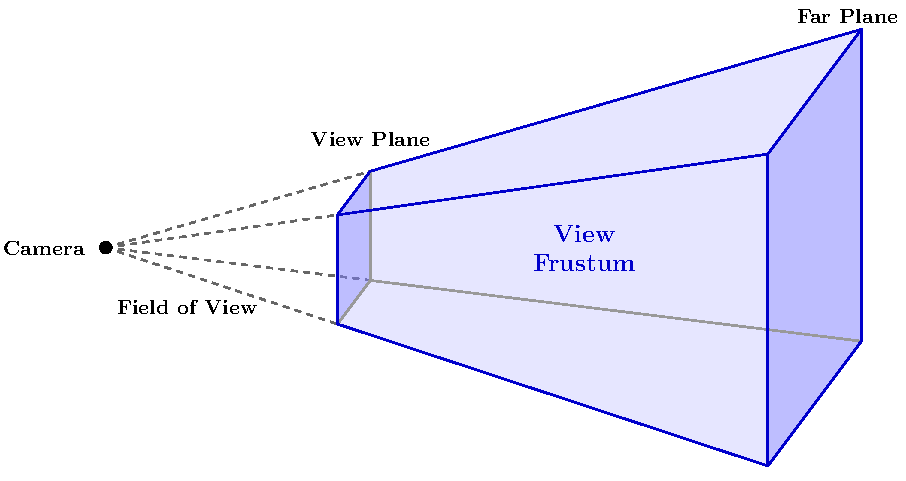
\includegraphics[width=0.8\textwidth]{../figures/view_frustum.pdf}
    \caption{A view frustum with the frustum in blue. Only elements inside the frustum between view and far planes are considered (own work).}
    \label{fig:view_frustum}
\end{figure}

\begin{figure}[H]
    \centering
    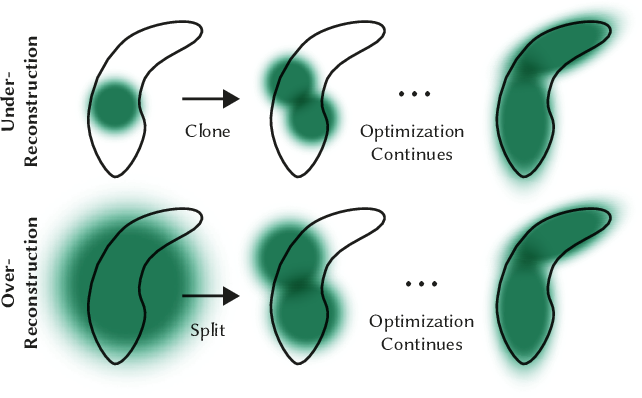
\includegraphics[width=0.7\textwidth]{../figures/6-Figure4-1.png}
    \caption{Adaptive Density Control situations for over- and under-reconstruction portraying cloning and splitting (taken from \cite{kerbl3DGaussianSplatting2023}).}
    \label{fig:adc}
\end{figure}

\newpage

\section{Full Backpropagation Calculations}

We skipped certain derivations in Chapter \ref{ch:backprop:phases} as their full calculations would be too long for this seminar paper format. We provide them here as they do not contribute much to the understanding of 3DGS backpropagation. Many of them rely on the trace operator $tr$ for matrix calculus, see \cite{riedel2025mathematische}. This is own work as no publications could be found dealing with math internals of 3DGS backpropagation.

\subsection{Phase 3: 2D Splat to 2D Geometry}
\label{ax:ph3}
To calculate $\frac{\partial \alpha_i}{\partial \Sigma_{2D}}$ we define $\alpha_i(p), \Delta$, exponent $E$ and vector $v$ as in Chapter \ref{ch:backprop:phases}, phase~3.

\paragraph{Step 1} Using the standard chain rule, we get: $$
\frac{\partial \alpha_i}{\partial \Sigma_{2D}} =
\frac{\partial \alpha_i}{\partial E} \cdot \frac{\partial E}{\partial \Sigma_{2D}}
,\hspace{3mm}\text{and}\hspace{3mm}\frac{\partial \alpha_i}{\partial E} = o \cdot \exp(E) = \alpha_i(p)
$$
This means we have to find the matrix derivative $\frac{\partial E}{\partial \Sigma_{2D}}$.

\paragraph{Step 2} The fundamental theorem of matrix calculus states that the differential $dE$ of a scalar function $E$ relates to its gradient matrix $\frac{\partial E}{\partial \Sigma_{2D}}$ via the trace operator ($\text{tr}$):
$$dE = \text{tr}\left( \left(\frac{\partial E}{\partial \Sigma_{2D}}\right)^T d\Sigma_{2D} \right)$$
If we can transform the differential of exponent $E$ into the form $\text{tr}(A^T d\Sigma_{2D})$, then the matrix $A$ is the derivative $\frac{\partial E}{\partial \Sigma_{2D}}$.

\paragraph{Step 3} Before we differentiate $E$, we must find the differential of the inverse matrix $\Sigma_{2D}^{-1}$. We begin with the basic identity property $\Sigma_{2D} \Sigma_{2D}^{-1} = I$ and take the differential of both sides using the product rule and rearrange further:
$$(d\Sigma_{2D}) \Sigma_{2D}^{-1} + \Sigma_{2D} (d\Sigma_{2D}^{-1}) = 0$$
$$\Sigma_{2D} (d\Sigma_{2D}^{-1}) = -(d\Sigma_{2D}) \Sigma_{2D}^{-1}$$
$$d\Sigma_{2D}^{-1} = -\Sigma_{2D}^{-1} (d\Sigma_{2D}) \Sigma_{2D}^{-1}$$

\paragraph{Step 4} Now we can take the differential of exponent $E$: $dE = -\frac{1}{2} \Delta p^T (d\Sigma_{2D}^{-1}) \Delta p$ and substituting from step 3 we get $$dE = \frac{1}{2} \Delta p^T \Sigma_{2D}^{-1} (d\Sigma_{2D}) \Sigma_{2D}^{-1} \Delta p$$

\paragraph{Step 5} Because $dE$ is a scalar value (a $1\times 1$ matrix), it is equal to its own trace: $dE = \text{tr}(dE)$. We apply the trace and utilize its cyclic permutation property, which allows us to shift matrices around inside the trace operator ($\text{tr}(ABC) = \text{tr}(CAB)$). Also, because covariance matrixes are strictly symmetric $(\Sigma_{2D}^{-1})^T = \Sigma_{2D}^{-1}$, we group the terms logically without needing to transpose matrices:
$$dE = \text{tr}\left( \frac{1}{2} \Delta p^T \Sigma_{2D}^{-1} (d\Sigma_{2D}) \Sigma_{2D}^{-1} \Delta p \right)$$
$$dE = \text{tr}\left( \frac{1}{2} \Delta p \Delta p^T \Sigma_{2D}^{-1} (d\Sigma_{2D}) \Sigma_{2D}^{-1} \right)$$
$$dE = \text{tr}\left( \left( \frac{1}{2} \Sigma_{2D}^{-1} \Delta p \Delta p^T \Sigma_{2D}^{-1} \right) d\Sigma_{2D} \right)$$

\paragraph{Step 6} Now we can match the rearranged trace equation to the identity rule from step~2 ($dE = \text{tr}(A^T d\Sigma_{2D})$), and extract matrix $A^T$:
$$A^T = \frac{1}{2} \Sigma_{2D}^{-1} \Delta p \Delta p^T \Sigma_{2D}^{-1}$$
Because the outer product of a vector with itself ($\Delta p \Delta p^T$) is symmetric, and multiplying it by symmetric inverse matrices on both sides maintains that symmetry, the entire block is symmetric. Therefore, $A^T = A$:
$$\frac{\partial E}{\partial \Sigma_{2D}} = \frac{1}{2} \Sigma_{2D}^{-1} \Delta p \Delta p^T \Sigma_{2D}^{-1}$$

\paragraph{Step 7} We substitute $v$: 
$$
\frac{\partial E}{\partial \Sigma_{2D}} =
\frac{1}{2} \left( \Sigma_{2D}^{-1} \Delta p \right) \left( \Delta p^T \Sigma_{2D}^{-1} \right) =
\frac{1}{2} v v^T
$$
and get
$$
\frac{\partial \alpha_i}{\partial \Sigma_{2D}} = 
\alpha_i(p) \cdot \frac{1}{2} v v^T =
\frac{1}{2} \alpha_i(p) \left( v v^T \right)
$$

\subsection{Phase 4: 2D Geometry to 3D Geometry}
\label{ax:ph4}
To calculate $\frac{\partial L}{\partial \Sigma_{3D}}$ we define $\Sigma_{2D} = U \Sigma_{3D} U^T$ and $U$ as in Chapter \ref{ch:backprop:phases}, phase~4.

\paragraph{Step 1} We already possess the upstream gradient $\frac{\partial L}{\partial \Sigma_{2D}}$ from the previous backpropagation phase. Calculating $\frac{\partial L}{\partial \Sigma_{3D}}$ makes again use of the trace operator.
$$
\text{Target:}\hspace{2mm}
dL = \text{tr}\left( \left(\frac{\partial L}{\partial \Sigma_{3D}}\right)^T d\Sigma_{3D} \right), 
\hspace{2mm}\text{and starting point}\hspace{2mm}
dL = \text{tr}\left( \left(\frac{\partial L}{\partial \Sigma_{2D}}\right)^T d\Sigma_{2D} \right).
$$

\paragraph{Step 2} We take the differential of the simplified forward pass equation. Because the projection matrix $U$ is independent of the 3D Gaussian covariance matrix, it acts as a constant during differentiation:$$d\Sigma_{2D} = U (d\Sigma_{3D}) U^T$$

\paragraph{Step 3} Now, we substitute this result for $d\Sigma_{2D}$ into the trace equation for $dL$:
$$dL = \text{tr}\left( \left(\frac{\partial L}{\partial \Sigma_{2D}}\right)^T U (d\Sigma_{3D}) U^T \right)$$
We apply the cyclic permutation property of the trace operator to shift the trailing $U^T$ from the right side of the expression to the front and group the terms multiplying $d\Sigma_{3D}$ into a single transposed block so we can extract the derivative.
$$dL = \text{tr}\left( U^T \left(\frac{\partial L}{\partial \Sigma_{2D}}\right)^T U (d\Sigma_{3D}) \right), \hspace{3mm}\text{and}\hspace{3mm}
U^T \left(\frac{\partial L}{\partial \Sigma_{2D}}\right)^T U =
\left( U^T \left(\frac{\partial L}{\partial \Sigma_{2D}}\right) U \right)^T
$$
Substituting this back into the target trace yields:
$$dL = \text{tr}\left( \left( U^T \frac{\partial L}{\partial \Sigma_{2D}} U \right)^T d\Sigma_{3D} \right)$$

\paragraph{Step 4} By matching the rearranged trace equation as in appendix \ref{ax:ph3}, we can directly extract gradient matrix $A$, yielding:
$$\frac{\partial L}{\partial \Sigma_{3D}} = U^T \left(\frac{\partial L}{\partial \Sigma_{2D}}\right) U$$

\subsection{Phase 5: 3D Geometry to 3D Gaussian Attributes}
\label{ax:ph5}

Phase 5 in Chapter \ref{ch:backprop:phases} is highly compressed, showing no direct calculations which we add here.

\subsubsection{Gradients for $M$, $S$, and $R$}

\paragraph{Step 1} We want to find $\frac{\partial L}{\partial M}$. Using the fundamental theorem of matrix calculus, the target template is $dL = \text{tr}\left( \left(\frac{\partial L}{\partial M}\right)^T dM \right)$ and the starting point (from the upstream gradient) is $dL = \text{tr}\left( \left(\frac{\partial L}{\partial \Sigma_{3D}}\right)^T d\Sigma_{3D} \right)$.

\paragraph{Step 2} We take the differential of $\Sigma_{3D} = M M^T$ using the product rule:
$$d\Sigma_{3D} = d(M M^T) = (dM) M^T + M (dM^T)$$
Because the differential and transpose operators are commutative, $d(M^T) = (dM)^T$:
$$d\Sigma_{3D} = (dM) M^T + M (dM)^T$$

\paragraph{Step 3} Substitute this into the starting trace equation:
$$dL = \text{tr}\left( \left(\frac{\partial L}{\partial \Sigma_{3D}}\right)^T \left( (dM) M^T + M (dM)^T \right) \right)$$
Using the linearity property of the trace operator ($\text{tr}(A + B) = \text{tr}(A) + \text{tr}(B)$), we split this into two separate terms:
$$dL = 
\text{tr}\left( \left(\frac{\partial L}{\partial \Sigma_{3D}}\right)^T (dM) M^T \right) + 
\text{tr}\left( \left(\frac{\partial L}{\partial \Sigma_{3D}}\right)^T M (dM)^T \right)
$$

\paragraph{Step 4} Because $\Sigma_{3D}$ is a valid covariance matrix, it is symmetric. Therefore, its gradient $\frac{\partial L}{\partial \Sigma_{3D}}$ is also strictly symmetric, meaning $\left(\frac{\partial L}{\partial \Sigma_{3D}}\right)^T = \frac{\partial L}{\partial \Sigma_{3D}}$. We transform both trace terms to isolate $dM$ on the right side:

First term: We use the cyclic permutation property to move $M^T$ to the front:
$$
\text{tr}\left( \frac{\partial L}{\partial \Sigma_{3D}} (dM) M^T \right) =
\text{tr}\left( M^T \frac{\partial L}{\partial \Sigma_{3D}} dM \right)
$$

Second term: We use the property that a matrix and its transpose share the same trace:\linebreak
$$
\text{tr}\left( \frac{\partial L}{\partial \Sigma_{3D}} M (dM)^T \right) =
\text{tr}\left( \left( \frac{\partial L}{\partial \Sigma_{3D}} M (dM)^T \right)^T \right)
$$
$$
= \text{tr}\left( dM M^T \frac{\partial L}{\partial \Sigma_{3D}} \right)
= \text{tr}\left( M^T \frac{\partial L}{\partial \Sigma_{3D}} dM \right)
$$

\paragraph{Step 5} As both terms are identical, we can add them together:
$$
dL = 2 \cdot \text{tr}\left( M^T \frac{\partial L}{\partial \Sigma_{3D}} dM \right) =
\text{tr}\left( \left(2 M^T \frac{\partial L}{\partial \Sigma_{3D}}\right) dM \right)
$$
Matching this against the target template $dL = \text{tr}(A^T dM)$, we extract the transpose:
$$\left(\frac{\partial L}{\partial M}\right)^T = 2 M^T \frac{\partial L}{\partial \Sigma_{3D}}$$
Transposing both sides yields the final result:
$$\frac{\partial L}{\partial M} = 2 \left(\frac{\partial L}{\partial \Sigma_{3D}}\right) M$$

\paragraph{Step 6} For $S$ and $R$, the new starting point uses the gradient we just calculated:
$$dL = \text{tr}\left( \left(\frac{\partial L}{\partial M}\right)^T dM \right)$$

\paragraph{Step 7} We apply the product rule to $M = R S$: $dM = (dR) S + R (dS)$ and substitute $dM$ into the trace:
$$dL = \text{tr}\left( \left(\frac{\partial L}{\partial M}\right)^T \left( (dR) S + R (dS) \right) \right)$$
We split it into two separate trace equations (since $S$ and $R$ are independent variables):
$$
dL_R = \text{tr}\left( \left(\frac{\partial L}{\partial M}\right)^T (dR) S \right),
\hspace{3mm}
dL_S = \text{tr}\left( \left(\frac{\partial L}{\partial M}\right)^T R (dS) \right)
$$

\paragraph{Step 8} For $R$, in the $dL_R$ equation, we use cyclic permutation to move $S$ to the front to isolate $dR$:
$$dL_R = \text{tr}\left( S \left(\frac{\partial L}{\partial M}\right)^T dR \right)$$
Matching this against the template $\text{tr}\left( \left(\frac{\partial L}{\partial R}\right)^T dR \right)$, we extract the transpose, transpose both sides and with $S^T = S$ we get:
$$
\left(\frac{\partial L}{\partial R}\right)^T = S \left(\frac{\partial L}{\partial M}\right)^T
\Leftrightarrow
\frac{\partial L}{\partial R} = \left(\frac{\partial L}{\partial M}\right) S^T
\Leftrightarrow
\frac{\partial L}{\partial R} = \left(\frac{\partial L}{\partial M}\right) S
$$

\paragraph{Step 9} For $S$, in the $dL_S$ equation, the differential $dS$ is already correctly isolated at the rear of the expression:
$$dL_S = \text{tr}\left( \left( \left(\frac{\partial L}{\partial M}\right)^T R \right) dS \right)$$
Matching this against the template $\text{tr}\left( \left(\frac{\partial L}{\partial S}\right)^T dS \right)$, we extract the transpose and transpose both sides:
$$
\left(\frac{\partial L}{\partial S}\right)^T = \left(\frac{\partial L}{\partial M}\right)^T R
\Leftrightarrow
\frac{\partial L}{\partial S} = R^T \left(\frac{\partial L}{\partial M}\right)
$$

\subsubsection{Gradients for 3D Covariance Matrix Components}

As gradients for the final scaling gradients have already been calculated in the chapter, we will focus on the gradients for the rotational quaternion ($q$ and $q_{raw}$).

We already possess the gradient $\frac{\partial L}{\partial R}$ from the previous step. To find the gradient of the loss with respect to each individual quaternion component $q_k$, $k \in \{w, x, y, z\}$, we use the chain rule combined with the trace operator. For each component, the scalar derivative is the Frobenius inner product ($\text{tr}(A^T B)$):
$$
\frac{\partial L}{\partial q_k} =
\text{tr}\left( \left(\frac{\partial L}{\partial R}\right)^T \frac{\partial R}{\partial q_k} \right) =
\sum_{i=1}^{3} \sum_{j=1}^{3} \left( \frac{\partial L}{\partial R} \right)_{ij} \left( \frac{\partial R}{\partial q_k} \right)_{ij}
$$
The partial derivative matrices $\frac{\partial R}{\partial q_k}$ are found by taking the element-wise derivative of the matrix $R$ (see Chapter \ref{ch:matrix_decomp}) with respect to $w, x, y,$ and $z$. These resolve to the following four constant matrices:
$$
\frac{\partial R}{\partial w} = 2 \begin{bmatrix} 0 & -z & y \\ z & 0 & -x \\ -y & x & 0 \end{bmatrix},
\hspace{5mm}
\frac{\partial R}{\partial x} = 2 \begin{bmatrix} 0 & y & z \\ y & -2x & -w \\ z & w & -2x \end{bmatrix}
$$
$$
\frac{\partial R}{\partial y} = 2 \begin{bmatrix} -2y & x & w \\ x & 0 & z \\ -w & z & -2y \end{bmatrix},
\hspace{5mm}
\frac{\partial R}{\partial z} = 2 \begin{bmatrix} -2z & -w & x \\ w & -2z & y \\ x & y & 0 \end{bmatrix}
$$
Evaluating the trace for all four components, e.g. $\frac{\partial L}{\partial w} = \text{tr}\left( \left(\frac{\partial L}{\partial R}\right)^T \frac{\partial R}{\partial w} \right)$, yields the $4 \times 1$ gradient vector $\frac{\partial L}{\partial q} = \begin{bmatrix} \vspace{1mm} \frac{\partial L}{\partial w} \\ \vspace{1mm} \frac{\partial L}{\partial x} \\ \vspace{1mm} \frac{\partial L}{\partial y} \\ \vspace{1mm} \frac{\partial L}{\partial z} \end{bmatrix}$.

\subsubsection{Gradient for Raw Quaternion}

During the forward pass, we normalized using $q = \frac{q_{raw}}{\vert{}\vert{}q_{raw}\vert{}\vert{}}$.

\paragraph{Step 1} Using the multi-variable chain rule, the gradient transforms via the Jacobian matrix of this normalization function:
$$\frac{\partial L}{\partial q_{raw}} = \left( \frac{\partial q}{\partial q_{raw}} \right)^T \frac{\partial L}{\partial q} = J_{\vert{}\vert{}}^T \frac{\partial L}{\partial q}$$

\paragraph{Step 2} To find $J_{\vert{}\vert{}}$, we must take the derivative of a vector divided by its own magnitude. To make this visually cleaner, we set $r = q_{raw}$, yielding $q = \frac{r}{\vert{}\vert{}r\vert{}\vert{}}$. 
We apply the quotient rule for vector differentiation:
$$
J_{\vert{}\vert{}} =
\frac{\partial}{\partial r} \left( \frac{r}{\vert{}\vert{}r\vert{}\vert{}} \right) =
\frac{\frac{\partial r}{\partial r} \vert{}\vert{}r\vert{}\vert{} - r \frac{\partial \vert{}\vert{}r\vert{}\vert{}}{\partial r}}{\vert{}\vert{}r\vert{}\vert{}^2}
$$
We evaluate the two numerator derivatives separately: The derivative of a vector with respect to itself is the identity matrix: $\frac{\partial r}{\partial r} = I$. The magnitude is defined as $\vert{}\vert{}r\vert{}\vert{} = (r^T r)^{1/2}$. Differentiating this using the chain rule yields:
$$
\frac{\partial \vert{}\vert{}r\vert{}\vert{}}{\partial r} =
\frac{1}{2} (r^T r)^{-1/2} (2 r^T) =
\frac{r^T}{(r^T r)^{1/2}} =
\frac{r^T}{\vert{}\vert{}r\vert{}\vert{}}
$$
Now, we substitute these two results back into the quotient rule equation:
$$
J_{\vert{}\vert{}} =
\frac{I \vert{}\vert{}r\vert{}\vert{} - r \left( \frac{r^T}{\vert{}\vert{}r\vert{}\vert{}} \right)}{\vert{}\vert{}r\vert{}\vert{}^2}
$$

\paragraph{Step 3} We split the fraction to simplify:
$$
J_{\vert{}\vert{}} =
\frac{I \vert{}\vert{}r\vert{}\vert{}}{\vert{}\vert{}r\vert{}\vert{}^2} - \frac{r r^T}{\vert{}\vert{}r\vert{}\vert{}^3}
\Leftrightarrow
J_{\vert{}\vert{}} =
\frac{I}{\vert{}\vert{}r\vert{}\vert{}} - \frac{r r^T}{\vert{}\vert{}r\vert{}\vert{}^3}
\Leftrightarrow J_{\vert{}\vert{}} = \frac{1}{\vert{}\vert{}r\vert{}\vert{}} \left( I - \frac{r r^T}{\vert{}\vert{}r\vert{}\vert{}^2} \right)
$$
The rightmost term can be rewritten as the outer product of the normalized vector with itself:
$$
\frac{r r^T}{\vert{}\vert{}r\vert{}\vert{}^2} =
\left( \frac{r}{\vert{}\vert{}r\vert{}\vert{}} \right) \left( \frac{r}{\vert{}\vert{}r\vert{}\vert{}} \right)^T =
q q^T
$$
Substituting this back in, and replacing $r$ with $q_{raw}$, we get the Jacobian:
$$
J_{\vert{}\vert{}} =
\frac{I - q q^T}{\vert{}\vert{}q_{raw}\vert{}\vert{}}
$$

\paragraph{Step 4} We return to the chain rule from step 1. Because the identity matrix $I$ is symmetric, and the outer product $q q^T$ is symmetric, their difference is symmetric. Dividing by a scalar $\vert{}\vert{}q_{raw}\vert{}\vert{}$ preserves this symmetry. Therefore, $J_{\vert{}\vert{}}^T = J_{\vert{}\vert{}}$, yielding the final equation that maps directly into the raw latent space:
$$
\frac{\partial L}{\partial q_{raw}} =
\frac{I - q q^T}{\vert{}\vert{}q_{raw}\vert{}\vert{}} \cdot \frac{\partial L}{\partial q}
$$

\subsubsection{Gradient for Base Opacity}

During the forward pass, the raw opacity $o_{raw}$ is passed through the sigmoid activation function: $\sigma(x) = \frac{1}{1 + e^{-x}}$. The derivative of $\sigma(x)$ is well-known and is $\sigma(x) \cdot (1 - \sigma(x))$.

We already possess the upstream gradient $\frac{\partial L}{\partial o}$ from phase 3. To find the gradient with respect to the raw opacity, we apply the chain rule and adjust the derivative of the sigmoid function for $o$:
$$
\frac{\partial L}{\partial o_{raw}} =
\frac{\partial L}{\partial o} \cdot \frac{\partial o}{\partial o_{raw}} =
\frac{\partial L}{\partial o} \cdot o (1 - o)
$$

\newpage